\chapter{Исследовательская часть}

В данном разделе приведены технические характеристики устройства, на котором проводились замеры времени выполнения программного обеспечения, а также результаты исследования.

\section{Технические характеристики}
Исследование по замерам времени выполнения программы проводились на персональном компьютере, оснащенном следующими компонентами:
\begin{itemize}
	\item процессор Intel Core i7-12700KF с 12 ядрами: 8 производительных и 4 энергоэффектиных, -- с суммарным числом потоков, равным 20~\cite{proc};
	\item оперативной памятью объемом 32~Гб;
	\item операционная система Windows 11 Home 64-рязрядная~\cite{win11}.
	\end{itemize}
	
\section{Описание исследования}
В рамках данного исследования проводятся замеры времени растеризации сцены в зависимости от числа используемых потоков. В исследовании участвуют две сцены: сцена с двумя сферами с коэффициентами отражения, равными 0.5, а также сцена с одной сферой с таким же коэффициентом зеркального отражения.

Для каждой сцены и каждого числа потоков рассчитывается и приводится медианное время по 50 замерам.

В рамках исследования по замерам времени использовался класс $Stopwatch$~\cite{Stopwatch} пространства имен $System.Diagnostics$~\cite{System.Diagnostics} языка программирования $C\#$~\cite{CSharp}.

\section{Результаты исследования}
Результаты исследования зависимости времени растеризации сцены объектов в зависимости от числа используемых потоков, приведены в таблице~\ref{tb:meas}.

\begin{table}[H]
	\begin{center}
		\begin{threeparttable}
			\centering
			\captionsetup{justification=raggedright,singlelinecheck=off}
			\caption{\label{tb:meas}Результаты исследования зависимости медианного времени растеризации сцены объектов в зависимости от числа используемых потоков}
			\begin{tabular}{| r | c | c |} \hline
				Число потоков & Сцена с одной сферой & Сцена с двумя сферами \\ \hline
				1 & 626.01 & 694.57 \\ \hline
				2 & 206.82 & 225.64 \\ \hline
				4 & 206.73 & 225.20 \\ \hline
				8 & 206.62 & 225.17 \\ \hline
				12 & 206.26 & 225.14 \\ \hline
				16 & 206.16 & 224.97 \\ \hline
				20 & 205.92 & 223.79 \\ \hline
				32 & 207.12 & 225.35 \\ \hline
				64 & 207.43 & 225.96 \\ \hline
			\end{tabular}
		\end{threeparttable}
	\end{center}
\end{table}


Результаты визуализации полученных данных приведены на рисунках~\ref{fig:meas}~-~\ref{fig:meas_scaled}.
\begin{figure}[H]
	\centering
	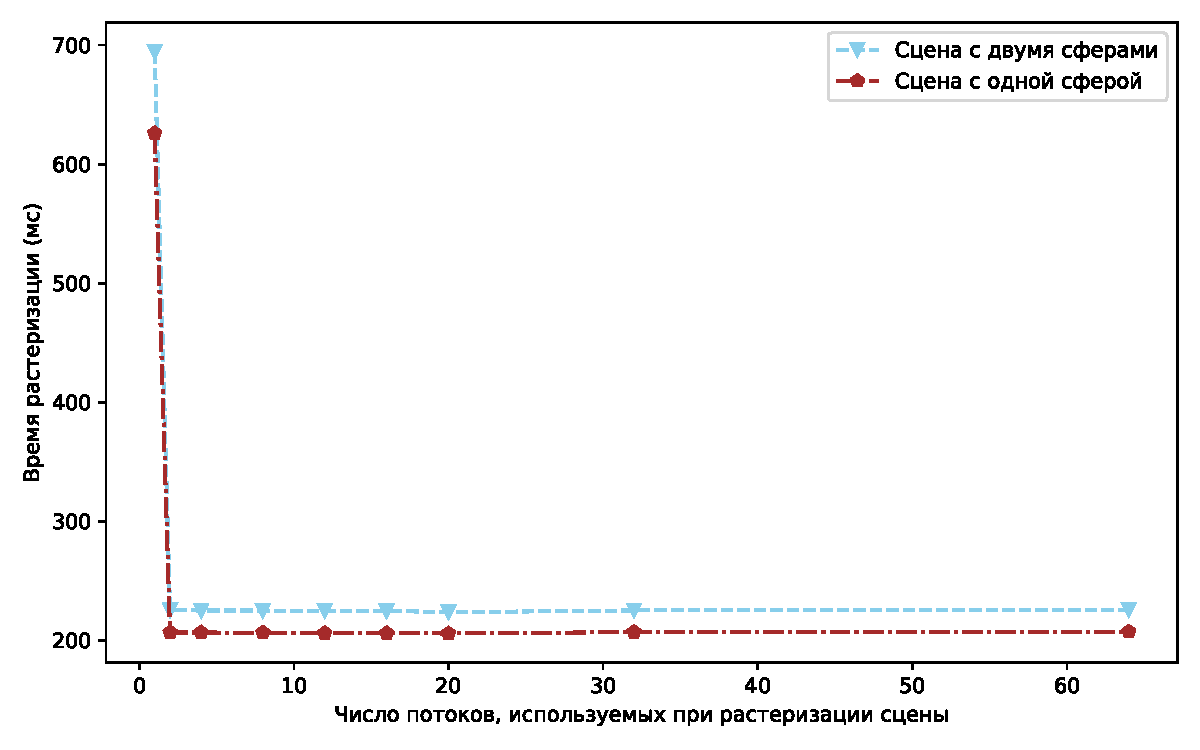
\includegraphics[width=0.8\textwidth]{spheres_time_measurements}
	\caption{График зависимости медианного времени растеризации сцены от числа используемых потоков}
	\label{fig:meas}
\end{figure}

\begin{figure}[H]
	\centering
	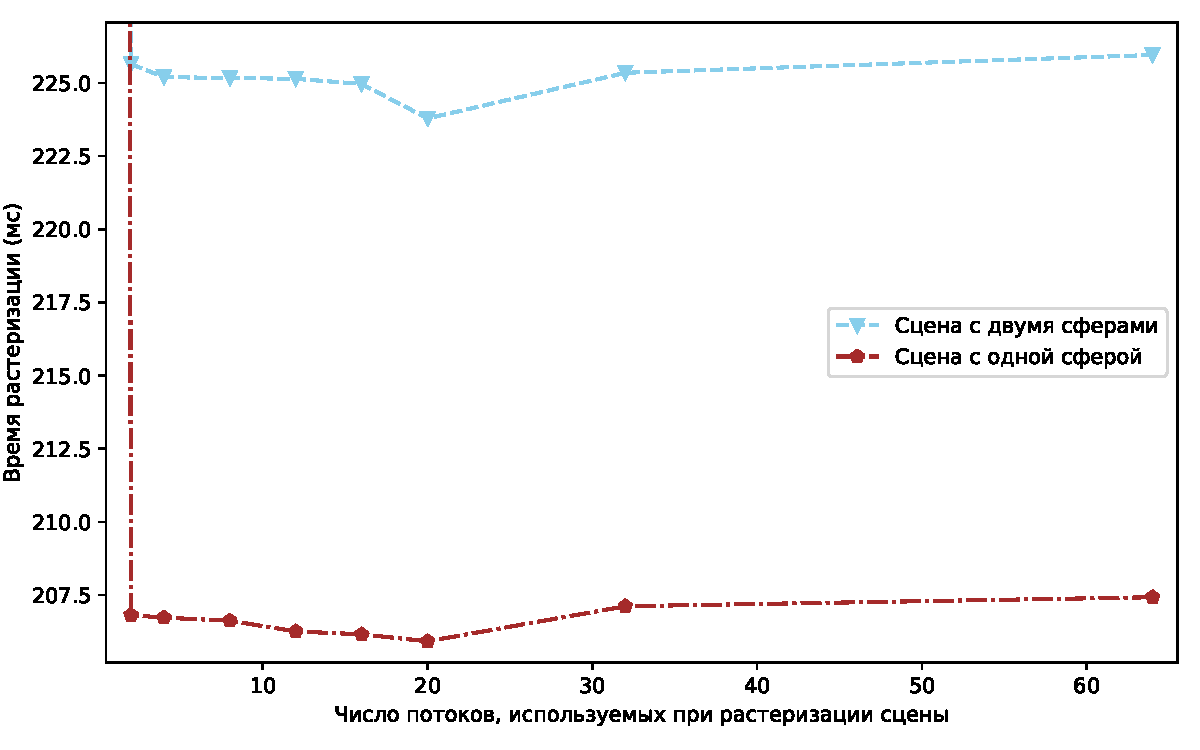
\includegraphics[width=0.8\textwidth]{spheres_time_measurements_scaled}
	\caption{График зависимости медианного времени растеризации сцены от числа используемых потоков (при числе потоков от 2 до 64)}
	\label{fig:meas_scaled}
\end{figure}

По результатам проведения замеров было установлено, что наиболее эффективным числом потоков для растеризации сцены является 20, это число совпало с числом потоков процессора. Использование большего числа потоков, чем позволяет процессор, приводит к увеличению времени выполнения программы, поскольку потоки выстраиваются в очередь, а также происходят более частые переключения контекста. При этом использование хотя бы двух потоков приводит к росту временной эффективности на 67-68\% относительно однопоточной версии программы. Результаты времени выполнения для 2 и 20 потоков различаются не более, чем на 0.5\%.

В ходе замеров было также выявлено, что при увеличении числа сфер на сцене от 1 до 2 время растеризации сцены увеличилось в среднем на 8.4\%.


\section*{Вывод}
В данном разделе было описано исследование замеров времени, описаны технические характеристики компьютера, на котором проводилось исследование, а также приведены результаты замеров. 

Результаты замерного эксперимента совпали с ожидаемыми: наиболее эффективным числом потоков является число потоков, аппаратно поддерживаемых процессором. Также в ходе эксперимента было подтверждено, что при увеличении числа объектов на сцене растет и время растеризации сцены (в случае с увеличением числа сфер от 1 до 2 рост составил 8.4\%).


\clearpage
